\documentclass[11pt,a4paper]{article}
\usepackage[utf8]{inputenc}
\usepackage[T1]{fontenc}
\usepackage{lmodern}
\usepackage[margin=2cm]{geometry}
\usepackage{amsmath,amssymb}
\usepackage{booktabs}
\usepackage{graphicx}
\usepackage{hyperref}
\usepackage{xcolor}
\usepackage{titlesec}
\usepackage{tabularx}
\usepackage{float}

\hypersetup{
    colorlinks=true,
    linkcolor=blue!70!black,
    citecolor=blue!70!black,
    urlcolor=blue!70!black
}

\titleformat{\section}{\large\bfseries}{\thesection.}{0.5em}{}
\titleformat{\subsection}{\normalsize\bfseries}{\thesubsection.}{0.5em}{}
\titlespacing*{\section}{0pt}{1.2ex plus 0.5ex minus .2ex}{0.6ex}
\titlespacing*{\subsection}{0pt}{1.0ex plus 0.4ex minus .2ex}{0.4ex}

\setlength{\parskip}{0.45em}
\setlength{\parindent}{0pt}

\begin{document}

\begin{center}
    {\LARGE \textbf{Projeto 2: Aprendizado Não Supervisionado}} \\[0.35em]
    {\large Disciplina: Introdução às Redes Neurais Artificiais} \\[0.3em]
    \textbf{Autor:} Vinícius Augusto Landim Andrade (RA: 169251) \\[0.2em]
    \textbf{Repositório / Código Reprodutível:} \url{https://github.com/vinicius-landim/neural-networks-course/project-2-SOM-GNG}
\end{center}
\vspace{-0.5em}
\hrule
\vspace{0.8em}

\section{Configuração Experimental}

Este trabalho investiga a redução do espaço de cores de imagens digitais por meio de duas redes neurais de aprendizado competitivo não supervisionado: o \textit{Self-Organizing Map} (SOM) e o \textit{Growing Neural Gas} (GNG). O objetivo é reduzir drasticamente a paleta de cada imagem, preservando a qualidade visual e a organização topológica do espaço de cores.

\subsection{Dados e reconstrução}

Cada imagem é tratada como um conjunto de dados tridimensional, em que cada
pixel é uma amostra com três características: os canais \textit{Red}, \textit{Green}
e \textit{Blue} (RGB). Os valores de cada canal são normalizados para o
intervalo $[0,1]$, de modo que um pixel é um vetor
$\mathbf{x}_i \in [0,1]^3$. Uma imagem de altura $H$ e largura $W$ é
reorganizada em uma matriz $\mathbf{X} \in \mathbb{R}^{N \times 3}$, com
$N = H \cdot W$, que é a entrada das redes.

Após o treinamento, cada neurônio da rede possui um vetor de pesos
$\mathbf{w}_k \in [0,1]^3$, que corresponde a uma cor da paleta final. A imagem é
reconstruída substituindo cada pixel pelo peso do seu neurônio vencedor, conhecido como \textit{Best Matching Unit} (BMU), em que seria o neurônio de menor distância
euclidiana ao pixel, conforme a Equação \ref{eq:dist}.
\begin{equation}
    \label{eq:dist}
  c(i) = \arg\min_{k} \left\lVert \mathbf{x}_i - \mathbf{w}_k \right\rVert,
  \qquad
  \hat{\mathbf{x}}_i = \mathbf{w}_{c(i)}.
\end{equation}
A matriz $\hat{\mathbf{X}}$ resultante é reorganizada em uma imagem
$H \times W \times 3$, que contém no máximo tantas cores distintas quanto o número
de neurônios da rede.

\subsection{Imagens e arquiteturas}

Foram utilizadas cinco imagens, todas recortadas para as dimensões
$900 \times 700$ pixels, o que resulta em $N = 630.000$ amostras por imagem. As imagens de treino são apresentadas na Figura \ref{fig:obras}.

\begin{figure}[H]
    \centering
    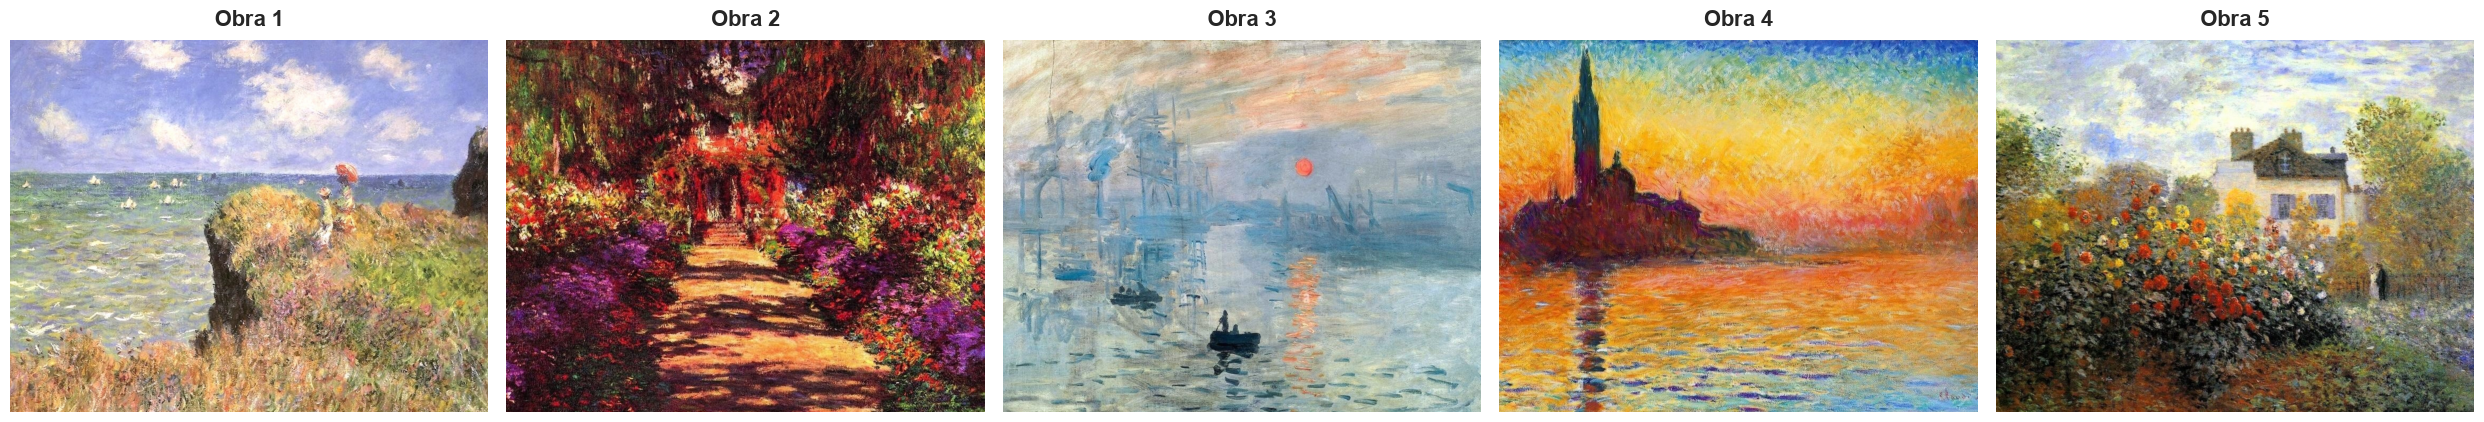
\includegraphics[width=\textwidth]{figs/obras.png}
    \caption{Imagens de treino.}
    \label{fig:obras}
\end{figure}

Para cada imagem, foram treinadas três configurações de cada rede, cujo número
de neurônios define o tamanho da paleta resultante:
\begin{itemize}
  \item \textbf{SOM:} grades retangulares de $4 \times 4$, $8 \times 8$ e
  $16 \times 16$ neurônios, o que equivale a paletas de 16, 64 e 256 cores;
  \item \textbf{GNG:} redes com 16, 64 e 256 neurônios, definidos como o
  número máximo de nós da rede.
\end{itemize}

\subsection{Métricas de avaliação}

O desempenho foi avaliado por quatro métricas, calculadas sobre todos os pixels
da imagem com os pesos finais de cada rede.

\paragraph{Erro de quantização (QE).} É a distância euclidiana média entre cada
pixel e o peso do seu BMU, no espaço RGB normalizado:
\begin{equation}
  \mathrm{QE} = \frac{1}{N} \sum_{i=1}^{N}
  \left\lVert \mathbf{x}_i - \mathbf{w}_{c(i)} \right\rVert .
\end{equation}
Quanto menor o QE, mais fiel é a paleta aos dados originais.

\paragraph{Erro topológico (TE).} É a fração de pixels cujo primeiro e
segundo BMU não são vizinhos na estrutura da rede:
\begin{equation}
  \mathrm{TE} = \frac{1}{N} \sum_{i=1}^{N} u_i,
  \qquad
  u_i =
  \begin{cases}
    1, & \text{se o 1º e o 2º BMU de } \mathbf{x}_i \text{ não são vizinhos},\\
    0, & \text{caso contrário.}
  \end{cases}
\end{equation}
No SOM, a vizinhança é definida pela grade (incluindo as posições diagonais).
No GNG, que não possui grade, dois neurônios são vizinhos quando estão
conectados por uma aresta. Por essa diferença, os valores de TE das duas redes
não são diretamente equivalentes. Quanto menor o TE, melhor a preservação
da topologia.

\paragraph{Erro quadrático médio (MSE).} É a média do quadrado das diferenças
entre a imagem original e a reconstruída, calculada sobre todos os pixels e
os três canais:
\begin{equation}
  \mathrm{MSE} = \frac{1}{3N} \sum_{i=1}^{N}
  \left\lVert \mathbf{x}_i - \hat{\mathbf{x}}_i \right\rVert^{2}.
\end{equation}

\paragraph{Relação sinal-ruído de pico (PSNR).} É expressa em decibéis (dB)
e, como os valores estão normalizados em $[0,1]$, o valor máximo do sinal é 1:
\begin{equation}
  \mathrm{PSNR} = 10 \log_{10} \left( \frac{1}{\mathrm{MSE}} \right).
\end{equation}
Quanto maior o PSNR, mais próxima a imagem reconstruída está da original.

\section{Rede SOM}

Os mapas auto-organizáveis foram implementados com a biblioteca
\textit{torchSOM}, com a configuração resumida na
Tabela~\ref{tab:som-config}. As métricas foram calculadas sobre todos os pixels
com os pesos finais, e o erro topológico considera vizinhas as oito células
adjacentes da grade (ortogonais e diagonais) e é apresentado em porcentagem. Cada
treinamento levou cerca de $61$ s, e nenhum neurônio ficou sem pixels associados
em qualquer configuração.

\begin{table}[htbp]
  \centering
  \small
  \begin{tabular}{ll}
    \toprule
    Parâmetro & Valor \\
    \midrule
    Topologia da grade & Retangular \\
    Tamanho da grade (neurônios) & $4 \times 4$ (16), $8 \times 8$ (64) e $16 \times 16$ (256) \\
    Função de vizinhança & Gaussiana \\
    Distância & Euclidiana \\
    Inicialização dos pesos & Aleatória \\
    Amostras de treinamento & Todos os pixels ($630.000$) \\
    Épocas & $30$ \\
    Tamanho do lote & $512$ \\
    Taxa de aprendizado inicial ($\eta_0$) & $0{,}5$, com decaimento inverso até zero \\
    Raio inicial da vizinhança ($\sigma_0$) & $2$, $4$ e $8$ (metade do lado da grade), com decaimento inverso até $1$ \\
    Semente aleatória & $42$ \\
    \bottomrule
    
  \end{tabular}
  \caption{Configuração dos mapas auto-organizáveis.}
  \label{tab:som-config}
\end{table}

Os resultados gerais estão na Tabela~\ref{tab:som-resultados}, com as métricas de
cada imagem e tamanho de grade. Em média, o aumento da grade reduziu de forma
consistente o erro de quantização e elevou o PSNR: o QE caiu de $0{,}1011$
($4 \times 4$) para $0{,}0570$ ($8 \times 8$) e $0{,}0380$ ($16 \times 16$), reduções
de cerca de $44\%$ e $33\%$ a cada quadruplicação da paleta, e o PSNR subiu de
$22{,}74$ para $27{,}53$ e $31{,}05$ dB. Isso ocorreu em todas as cinco imagens. O
melhor resultado do conjunto foi o de Obra 3 na grade
$16 \times 16$ ($\mathrm{QE} = 0{,}0245$; $\mathrm{PSNR} = 32{,}93$ dB), e o pior foi o de
Obra 4 na grade $4 \times 4$
($\mathrm{QE} = 0{,}1264$; $\mathrm{PSNR} = 21{,}34$ dB). O erro topológico se manteve
baixo em todos os casos, com máximo de $3{,}11\%$, e ficou abaixo de $1\%$ em nove
das quinze configurações. Diferentemente do QE, o TE médio não diminuiu com o
tamanho da grade ($0{,}90\%$, $1{,}03\%$ e $1{,}19\%$).

\begin{table}[H]
  \centering
  \small
  \begin{tabular}{llcccc}
    \toprule
    Imagem & Grade & QE & TE (\%) & MSE ($\times 10^{-3}$) & PSNR (dB) \\
    \midrule
    Obra 1
      & $4 \times 4$   & 0{,}1033 & 0{,}011 & 5{,}438 & 22{,}65 \\
      & $8 \times 8$   & 0{,}0537 & $<0{,}001$ & 1{,}497 & 28{,}25 \\
      & $16 \times 16$ & 0{,}0343 & 0{,}398 & 0{,}616 & 32{,}10 \\
    \midrule
    Obra 2
      & $4 \times 4$   & 0{,}1005 & 1{,}398 & 5{,}532 & 22{,}57 \\
      & $8 \times 8$   & 0{,}0627 & 1{,}979 & 2{,}174 & 26{,}63 \\
      & $16 \times 16$ & 0{,}0454 & 2{,}561 & 1{,}178 & 29{,}29 \\
    \midrule
    Obra 3
      & $4 \times 4$   & 0{,}0698 & 0{,}097 & 3{,}635 & 24{,}40 \\
      & $8 \times 8$   & 0{,}0394 & 0{,}058 & 1{,}371 & 28{,}63 \\
      & $16 \times 16$ & 0{,}0245 & 0{,}223 & 0{,}510 & 32{,}93 \\
    \midrule
    Obra 4
      & $4 \times 4$   & 0{,}1264 & 0{,}000 & 7{,}349 & 21{,}34 \\
      & $8 \times 8$   & 0{,}0739 & 0{,}000 & 2{,}492 & 26{,}03 \\
      & $16 \times 16$ & 0{,}0508 & 0{,}261 & 1{,}212 & 29{,}16 \\
    \midrule
    Obra 5
      & $4 \times 4$   & 0{,}1055 & 3{,}017 & 5{,}329 & 22{,}73 \\
      & $8 \times 8$   & 0{,}0554 & 3{,}109 & 1{,}545 & 28{,}11 \\
      & $16 \times 16$ & 0{,}0352 & 2{,}484 & 0{,}667 & 31{,}76 \\
    \midrule
    \textbf{Média}
      & $4 \times 4$   & 0{,}1011 & 0{,}904 & 5{,}457 & 22{,}74 \\
      & $8 \times 8$   & 0{,}0570 & 1{,}029 & 1{,}816 & 27{,}53 \\
      & $16 \times 16$ & 0{,}0380 & 1{,}185 & 0{,}837 & 31{,}05 \\
    \bottomrule
  \end{tabular}
  \caption{Métricas do SOM para cada imagem e tamanho de grade, calculadas
  sobre todos os pixels. O TE está em porcentagem e o MSE em unidades de $10^{-3}$.}
  \label{tab:som-resultados}
\end{table}

\begin{figure}[H]
    \centering
    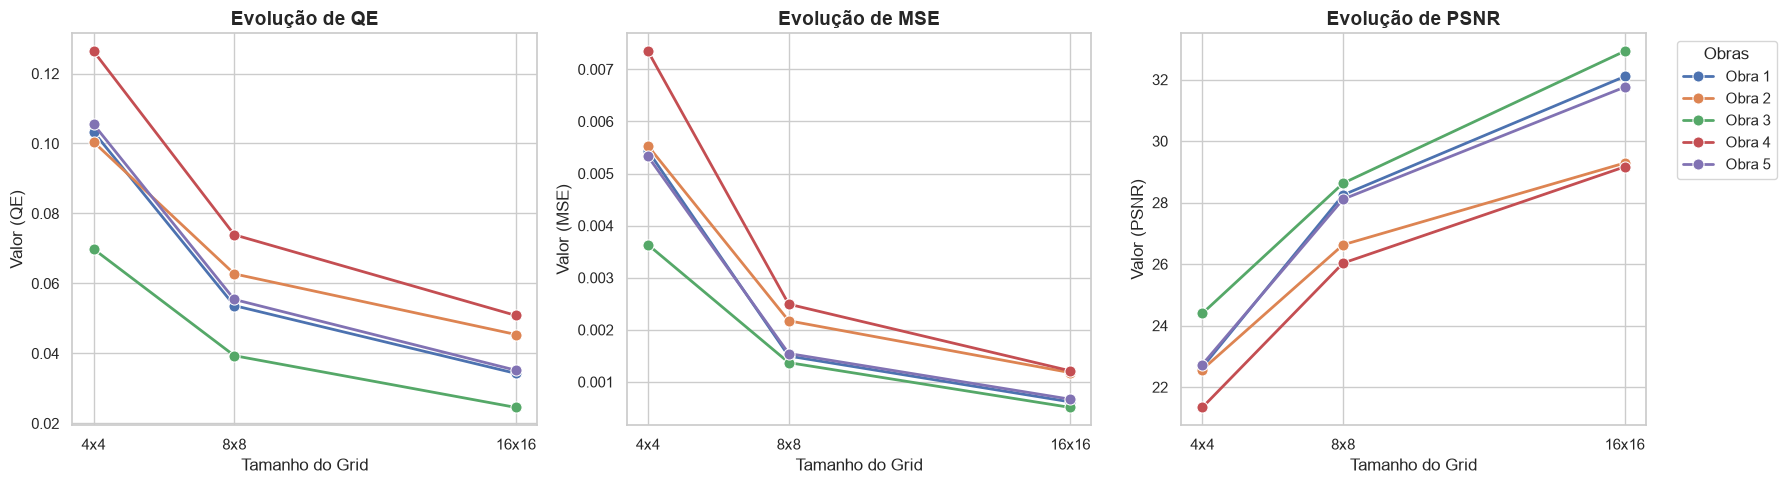
\includegraphics[width=\textwidth]{figs/som/evolucao-metricas.png}
    \caption{Evolução das métricas QE, MSE e PSNR pelo tamanho do grid para cada imagem.}
    \label{fig:som-grid-metricas}
\end{figure}

A Figura~\ref{fig:som-grid-metricas} apresenta cada métrica em função do
tamanho da grade, com uma curva por imagem. O QE e o MSE diminuíram e o PSNR
aumentou em todas as imagens, mas com retornos decrescentes: o ganho de PSNR foi
maior na passagem de $4 \times 4$ para $8 \times 8$ (de $4{,}06$ a $5{,}60$ dB) do que de
$8 \times 8$ para $16 \times 16$ (de $2{,}66$ a $4{,}30$ dB), com exceção de
Obra 3, em que os dois ganhos foram praticamente iguais
($4{,}23$ e $4{,}30$ dB). A Obra 3 teve sempre o menor QE e a
Obra 4 o maior ao longo das grades, e a ordenação completa das imagens se manteve
entre as grades $8 \times 8$ e $16 \times 16$. A razão entre o maior e o menor QE
cresceu de $1{,}81$ ($4 \times 4$) para $2{,}07$ ($16 \times 16$). A Obra 2 teve o menor ganho total de PSNR ($6{,}72$ dB), contra $9{,}46$ dB em
Obra 1. O TE teve comportamento menos uniforme:
As Obras 1, 3 e 4 ficaram
abaixo de $0{,}4\%$ e aumentaram na maior grade, a Obra 2 cresceu a cada
aumento da grade ($1{,}40\%$ a $2{,}56\%$), e Obra 5
manteve os maiores valores ($2{,}48\%$ a $3{,}11\%$), diminuindo na grade
$16 \times 16$.

As Figuras ~\ref{fig:som-obra1}, \ref{fig:som-obra2}, \ref{fig:som-obra3}, \ref{fig:som-obra4} e \ref{fig:som-obra5} mostram, para cada pintura, a imagem original e as reconstruções com paletas de $16$, $64$ e $256$ cores, junto das paletas correspondentes, dispostas na
própria grade do SOM. Como nenhum neurônio ficou sem pixels associados, todas as
cores de cada paleta foram usadas na reconstrução. Além disso, os baixos valores
de TE indicam que neurônios vizinhos na grade tendem a ter cores semelhantes, o
que se reflete na organização das paletas.

\begin{figure}[H]
    \centering
    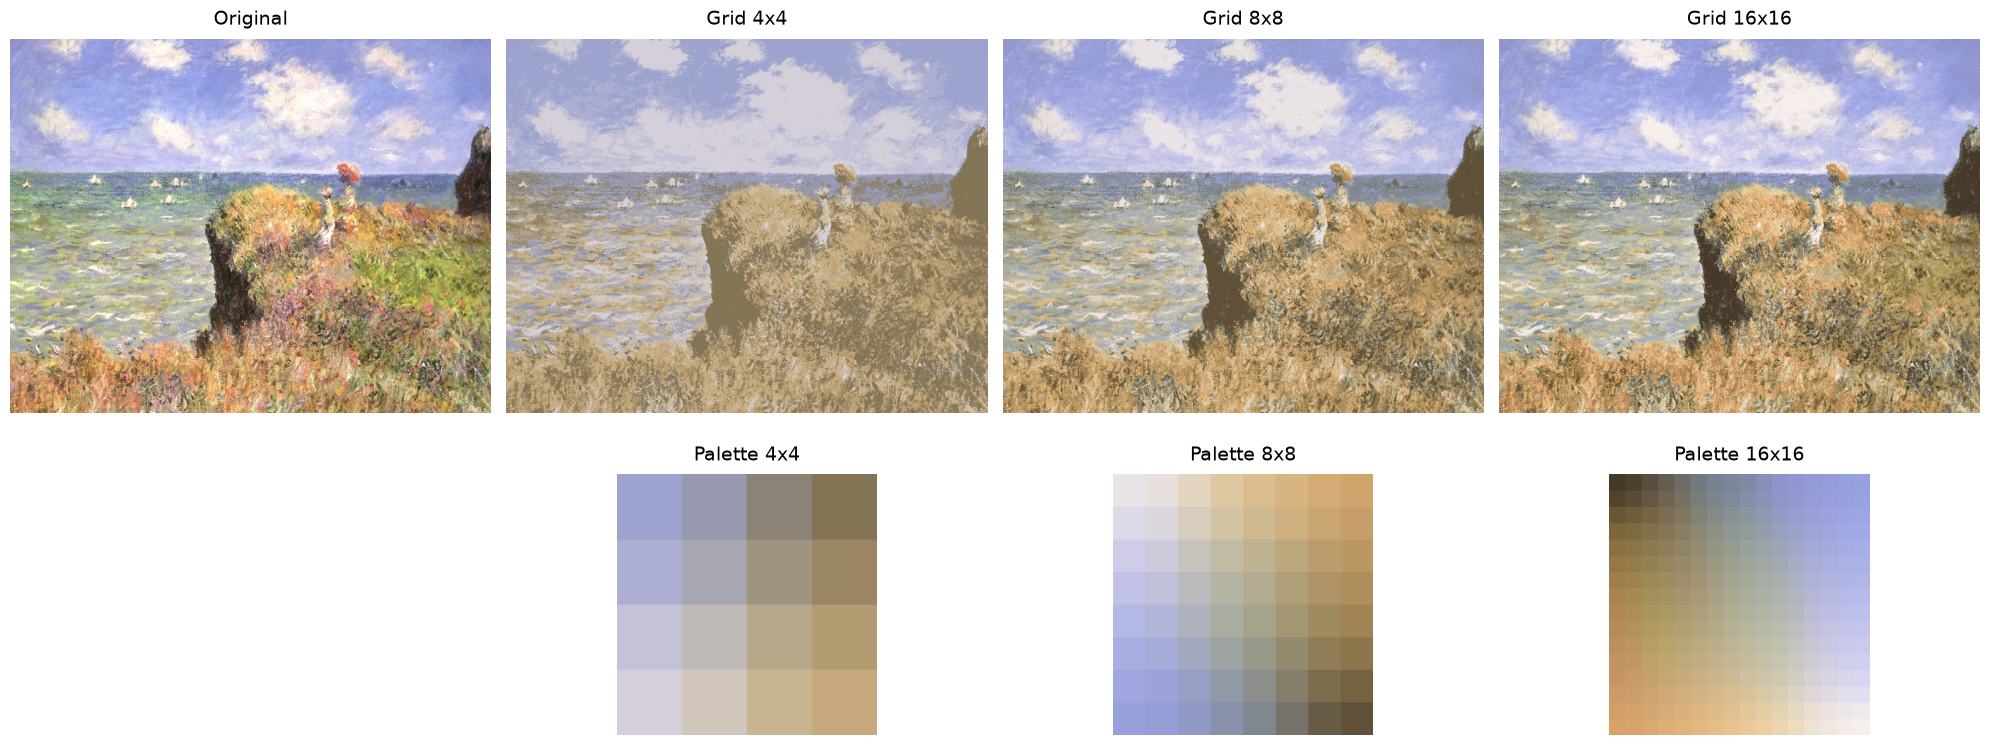
\includegraphics[width=\textwidth]{figs/som/result-cliff-walk-at-pourville.png}
    \caption{Reconstrução da Obra 1 com paleta obtida com o grid da rede SOM} \label{fig:som-obra1}
\end{figure}

\begin{figure}[H]
    \centering
    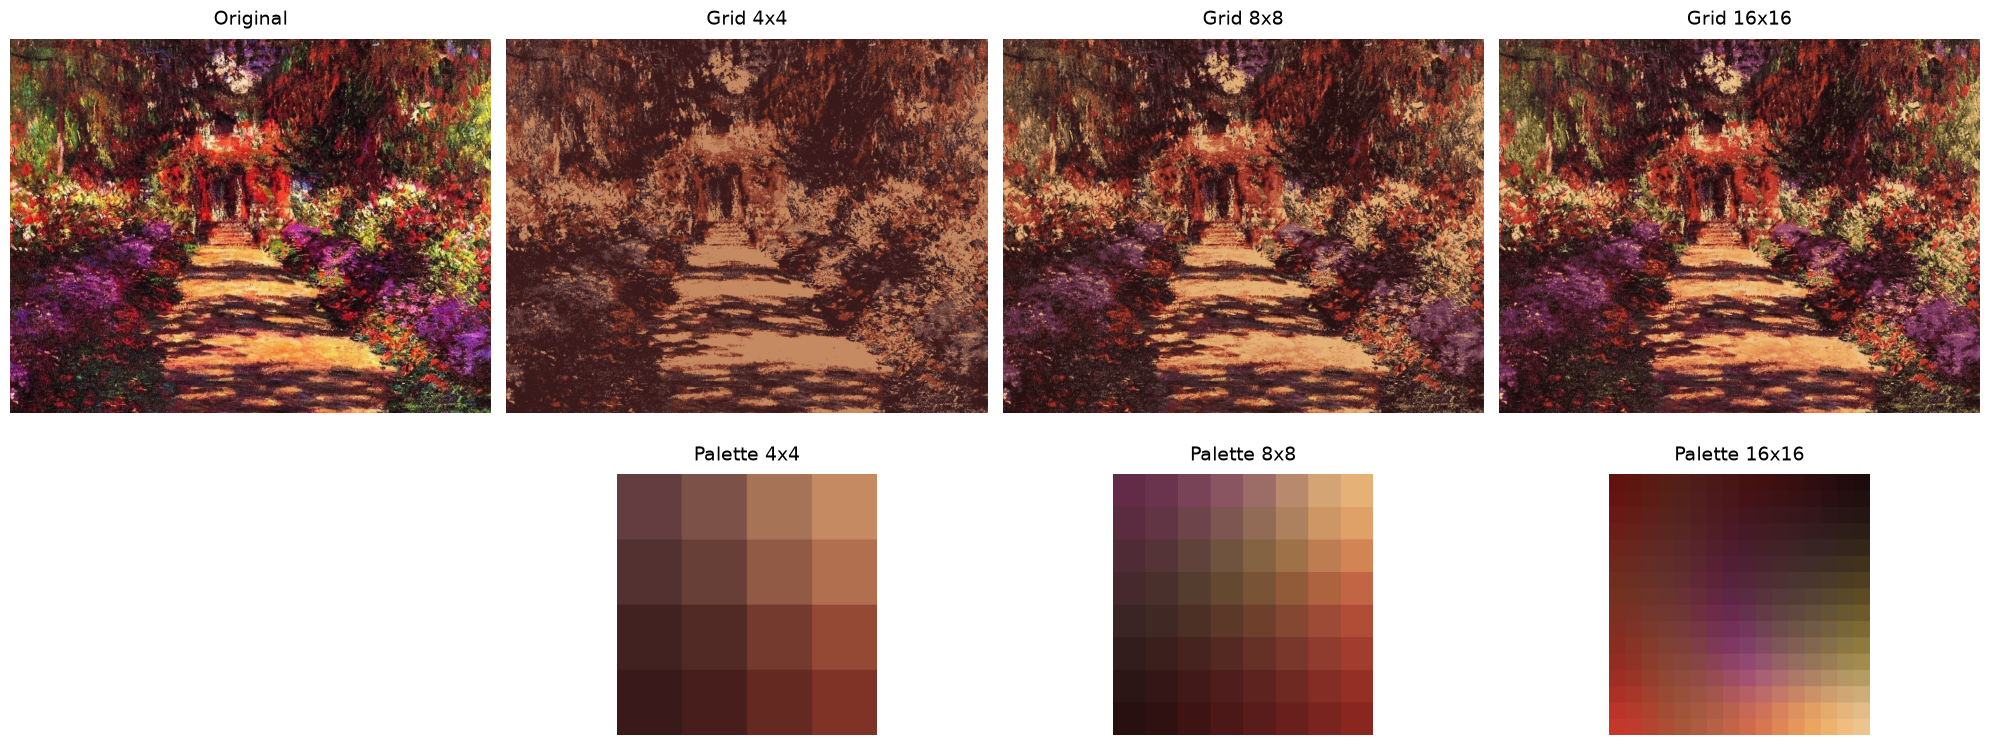
\includegraphics[width=\textwidth]{figs/som/result-garden-path-at-giverny.png}
    \caption{Reconstrução da Obra 2 com paleta obtida com o grid da rede SOM} \label{fig:som-obra2}
\end{figure}

\begin{figure}[H]
    \centering
    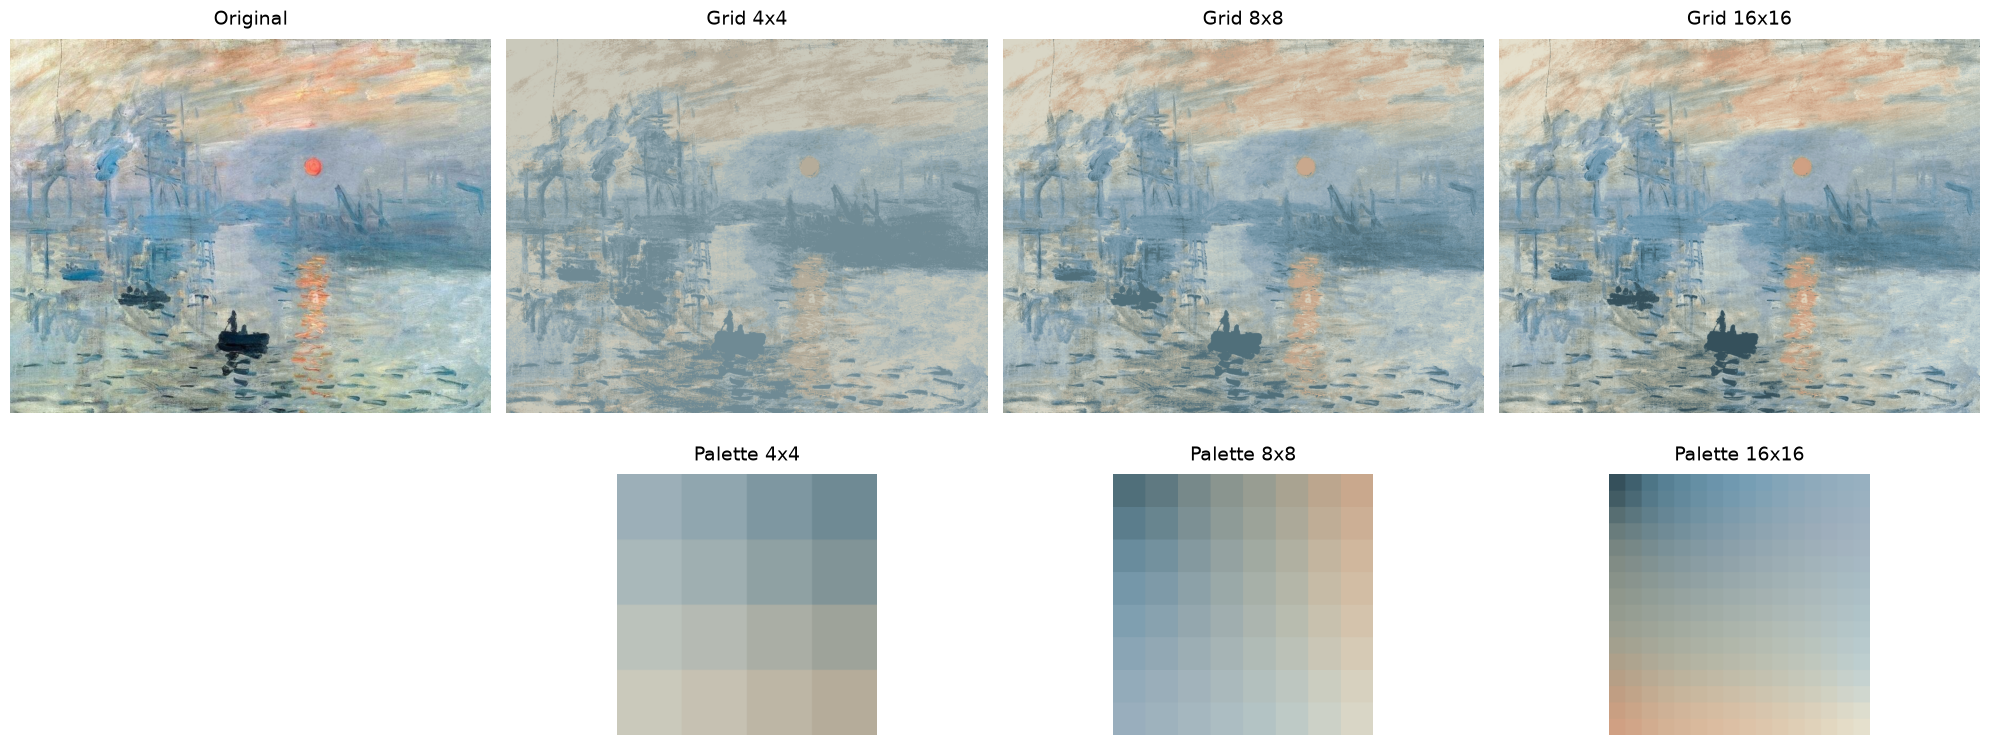
\includegraphics[width=\textwidth]{figs/som/results-impression-sunrise.png}
    \caption{Reconstrução da Obra 3 com paleta obtida com o grid da rede SOM} \label{fig:som-obra3}
\end{figure}

\begin{figure}[H]
    \centering
    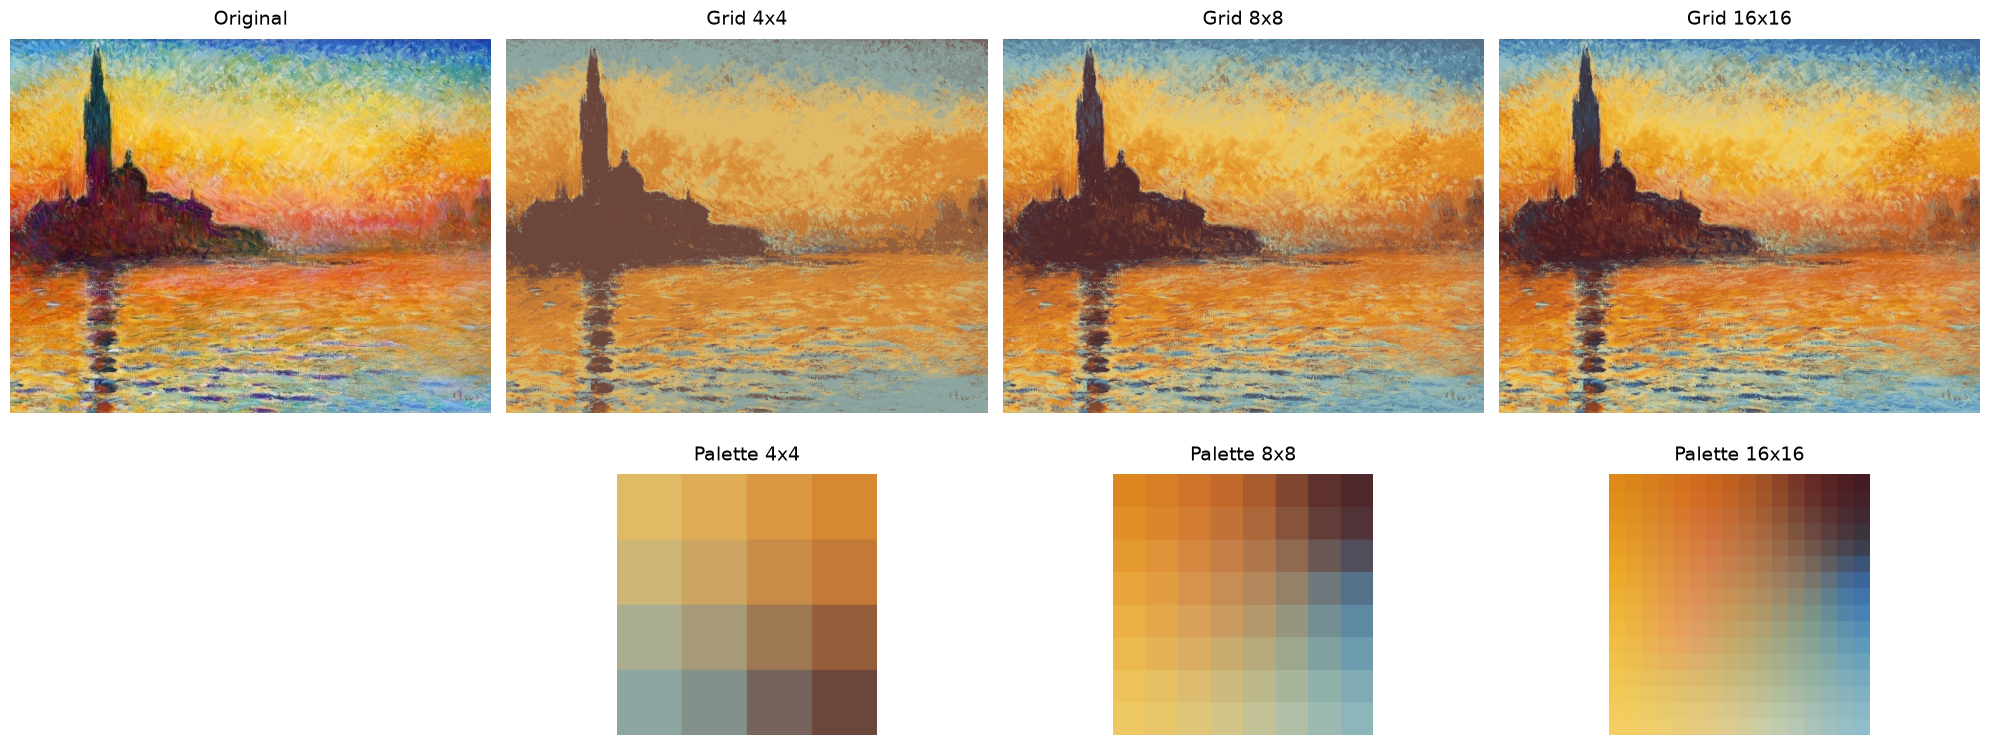
\includegraphics[width=\textwidth]{figs/som/results-san-giorgio-maggiore-at-dusk.png}
    \caption{Reconstrução da Obra 4 com paleta obtida com o grid da rede SOM} \label{fig:som-obra4}
\end{figure}

\begin{figure}[H]
    \centering
    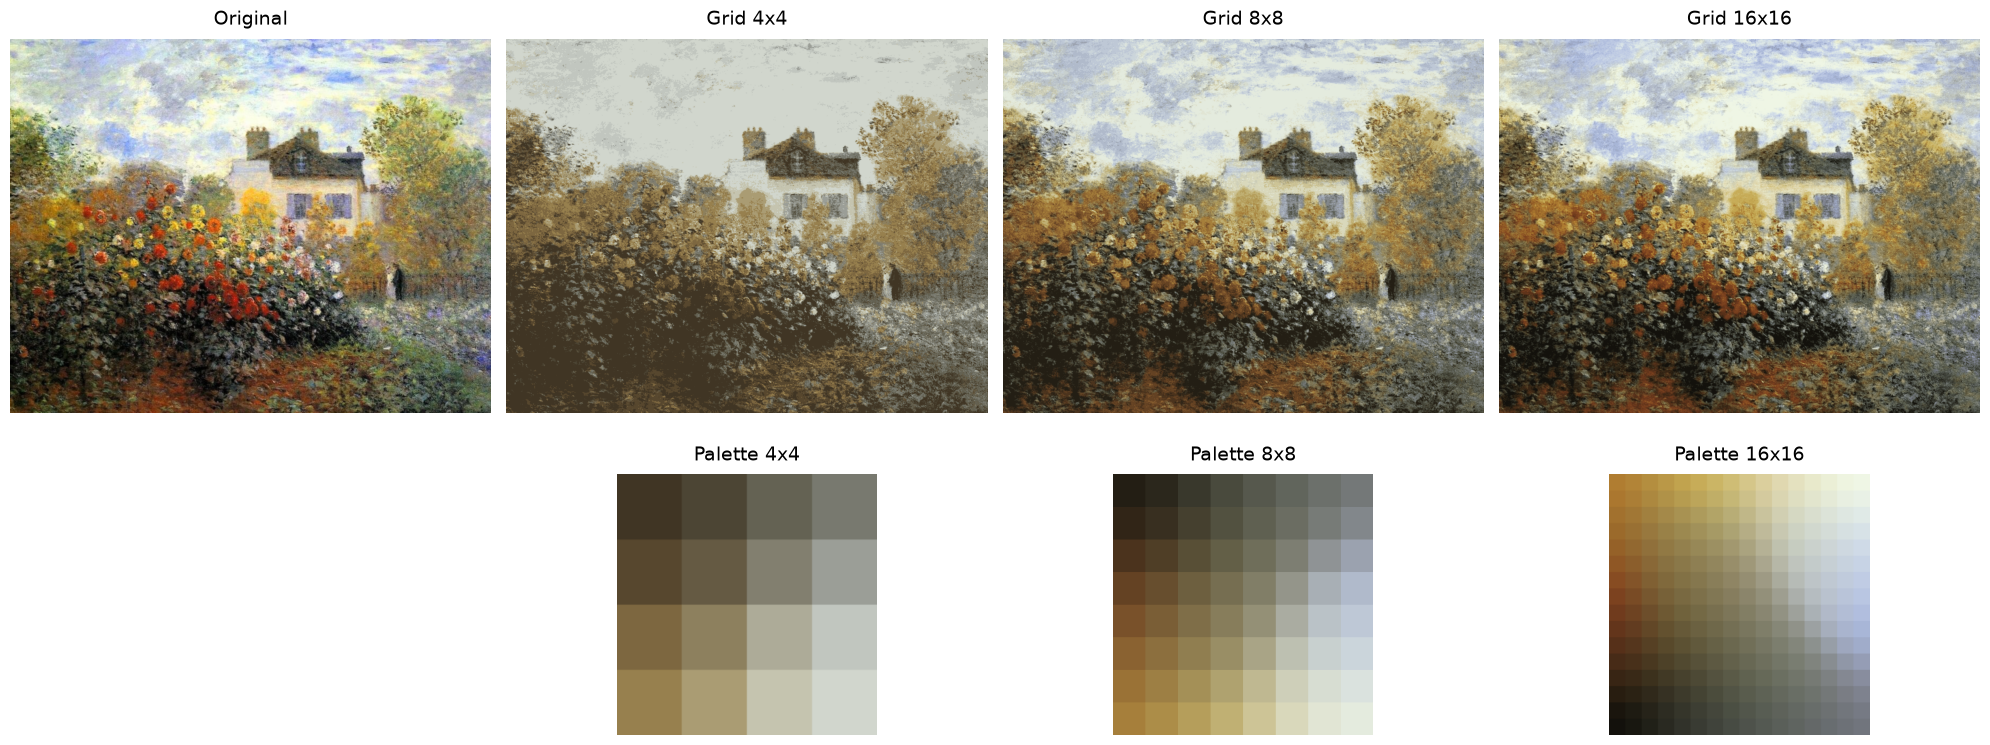
\includegraphics[width=\textwidth]{figs/som/results-the-garden-of-monet-at-argenteuil.png}
    \caption{Reconstrução da Obra 5 com paleta obtida com o grid da rede SOM} \label{fig:som-obra5}
\end{figure}

De maneira geral, para os grids menores, observou-se uma menor representatividade de tons de cores e gradações notáveis ao longo da imagem. Na medida em que se aumentaram o tamanho do grid, essas características se reduziram.
% CONFERIR NAS FIGURAS: perda de gradações (\textit{banding}) com $16$ cores,
% cores raras que sumiram (por exemplo, tons de menor área), e quão suave é a
% organização das paletas, em especial para Argenteuil e Garden Path (TE mais
% alto). Incluir aqui uma ou duas frases com o que for visível.

\section{Rede GNG}

A rede \textit{Growing Neural Gas} foi implementada em Python com NumPy, com a
configuração resumida na Tabela~\ref{tab:gng-config}. A rede parte de dois
neurônios inicializados com pixels sorteados da imagem e insere um novo neurônio
a cada $\lambda = 50$ iterações, até atingir o número máximo de nós $K$ ($16$,
$64$ ou $256$). A partir daí, o treinamento prossegue apenas com o ajuste dos
pesos. O treinamento usou todos os pixels de cada imagem ($630.000$ amostras)
em uma única época, o que corresponde a $630.000$ iterações. Para $K = 256$, a
rede completa a fase de crescimento em cerca de $12.700$ iterações
($(256-2) \times 50$), sendo o
restante das iterações operando como ajuste fino. Em todas as quinze configurações, a rede terminou com
exatamente $K$ neurônios, e nenhum ficou sem pixels associados. As métricas
foram calculadas sobre todos os pixels com os pesos finais. O erro topológico
considera vizinhos os neurônios conectados por uma aresta e é apresentado em
porcentagem. Como o algoritmo cria uma aresta entre os dois neurônios mais
próximos a cada amostra apresentada, o TE tende a ser baixo por construção.
Cada treinamento levou, em média, $35$ s ($K = 16$), $93$ s ($K = 64$) e
$325$ s ($K = 256$).

\begin{table}[htbp]
  \centering
  \small
  \begin{tabular}{ll}
    \toprule
    Parâmetro & Valor \\
    \midrule
    Número máximo de neurônios ($K$) & $16$, $64$ e $256$ \\
    Neurônios iniciais & $2$ (pixels sorteados da imagem) \\
    Taxa de aprendizado do vencedor ($\eta_b$) & $0{,}1$ \\
    Taxa de aprendizado dos vizinhos ($\eta_n$) & $0{,}001$ \\
    Idade máxima das arestas & $90$ \\
    Intervalo de inserção de neurônios ($\lambda$) & $50$ iterações \\
    Redução do erro dos neurônios na inserção ($\alpha$) & $0{,}5$ \\
    Decaimento do erro por iteração ($\beta$) & $0{,}005$ \\
    Épocas & $1$ \\
    Amostras de treinamento & Todos os pixels ($630.000$) \\
    Semente aleatória & $42$ \\
    \bottomrule
  \end{tabular}
  \caption{Configuração das redes \textit{Growing Neural Gas}.}
  \label{tab:gng-config}
\end{table}

Os resultados gerais estão na Tabela~\ref{tab:gng-resultados}, com as métricas de
cada imagem e número de neurônios. Em média, o aumento da rede reduziu de forma
consistente o erro de quantização e elevou o PSNR: o QE caiu de $0{,}0746$
($K = 16$) para $0{,}0450$ ($K = 64$) e $0{,}0283$ ($K = 256$), reduções de cerca
de $40\%$ e $37\%$ a cada quadruplicação da paleta, e o PSNR subiu de $26{,}51$
para $31{,}01$ e $35{,}06$ dB. Isso ocorreu em todas as cinco imagens. O melhor
resultado do conjunto foi o da Obra 3 com $K = 256$ ($\mathrm{QE} = 0{,}0180$;
$\mathrm{PSNR} = 38{,}75$ dB), e o pior foi o da Obra 4 com $K = 16$
($\mathrm{QE} = 0{,}0957$; $\mathrm{PSNR} = 24{,}49$ dB). O erro topológico se
manteve baixo em todos os casos, com máximo de $1{,}59\%$ (Obra 2, $K = 64$), e
ficou abaixo de $1\%$ em doze das quinze configurações. O TE médio aumentou com o
tamanho da rede ($0{,}10\%$, $0{,}59\%$ e $1{,}02\%$).

\begin{table}[H]
  \centering
  \small
  \begin{tabular}{llcccc}
    \toprule
    Imagem & $K$ & QE & TE (\%) & MSE ($\times 10^{-3}$) & PSNR (dB) \\
    \midrule
    Obra 1
      & $16$  & 0{,}0707 & 0{,}277 & 2{,}012 & 26{,}96 \\
      & $64$  & 0{,}0420 & 0{,}642 & 0{,}724 & 31{,}41 \\
      & $256$ & 0{,}0261 & 0{,}729 & 0{,}281 & 35{,}52 \\
    \midrule
    Obra 2
      & $16$  & 0{,}0792 & 0{,}100 & 2{,}792 & 25{,}54 \\
      & $64$  & 0{,}0506 & 1{,}593 & 1{,}090 & 29{,}63 \\
      & $256$ & 0{,}0323 & 1{,}328 & 0{,}449 & 33{,}47 \\
    \midrule
    Obra 3
      & $16$  & 0{,}0512 & 0{,}015 & 1{,}159 & 29{,}36 \\
      & $64$  & 0{,}0294 & 0{,}179 & 0{,}360 & 34{,}44 \\
      & $256$ & 0{,}0180 & 0{,}818 & 0{,}133 & 38{,}75 \\
    \midrule
    Obra 4
      & $16$  & 0{,}0957 & 0{,}072 & 3{,}554 & 24{,}49 \\
      & $64$  & 0{,}0582 & 0{,}389 & 1{,}331 & 28{,}76 \\
      & $256$ & 0{,}0371 & 1{,}415 & 0{,}544 & 32{,}64 \\
    \midrule
    Obra 5
      & $16$  & 0{,}0764 & 0{,}016 & 2{,}400 & 26{,}20 \\
      & $64$  & 0{,}0448 & 0{,}135 & 0{,}830 & 30{,}81 \\
      & $256$ & 0{,}0280 & 0{,}788 & 0{,}324 & 34{,}89 \\
    \midrule
    \textbf{Média}
      & $16$  & 0{,}0746 & 0{,}096 & 2{,}384 & 26{,}51 \\
      & $64$  & 0{,}0450 & 0{,}587 & 0{,}867 & 31{,}01 \\
      & $256$ & 0{,}0283 & 1{,}016 & 0{,}346 & 35{,}06 \\
    \bottomrule
  \end{tabular}
  \caption{Métricas da GNG para cada imagem e número de neurônios, calculadas
  sobre todos os pixels.}
  \label{tab:gng-resultados}
\end{table}

\begin{figure}[H]
    \centering
    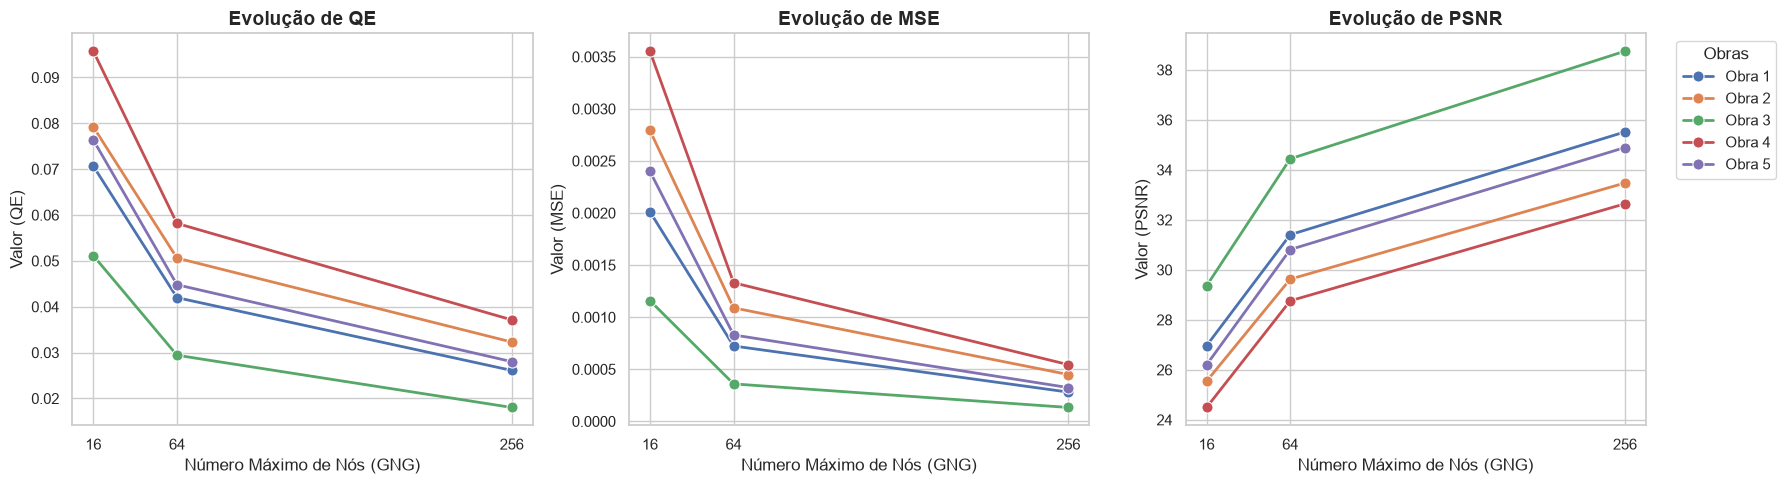
\includegraphics[width=\textwidth]{figs/gng/evolucao-metricas.png}
    \caption{Evolução das métricas QE, MSE e PSNR pelo número de K neurônios na rede GNG.}
    \label{fig:gng-grid-metricas}
\end{figure}

A Figura~\ref{fig:gng-grid-metricas} apresenta cada métrica em função do número
de neurônios, com uma curva por imagem. O QE e o MSE diminuíram e o PSNR aumentou
em todas as imagens, com retornos decrescentes: o ganho de PSNR foi maior na
passagem de $K = 16$ para $K = 64$ (de $4{,}09$ a $5{,}08$ dB) do que de $K = 64$
para $K = 256$ (de $3{,}85$ a $4{,}31$ dB) em todas as imagens. A ordenação das
imagens por QE se manteve em todos os tamanhos de rede, com a Obra 3 sempre no
menor valor e a Obra 4 no maior, e a razão entre os dois cresceu de $1{,}87$
($K = 16$) para $2{,}06$ ($K = 256$). A Obra 3 teve o maior ganho total de PSNR
($9{,}39$ dB) e a Obra 2, o menor ($7{,}93$ dB). O TE aumentou a cada aumento da
rede nas Obras 1, 3, 4 e 5 (por exemplo, de $0{,}07\%$ para $1{,}42\%$ na Obra 4),
enquanto a Obra 2 atingiu o máximo do conjunto em $K = 64$ ($1{,}59\%$) e diminuiu
em $K = 256$ ($1{,}33\%$).

% >>> Figuras fig:gng-obra1 ... fig:gng-obra5 (reconstruções e paletas) aqui

As Figuras~\ref{fig:gng-obra1}, \ref{fig:gng-obra2}, \ref{fig:gng-obra3},
\ref{fig:gng-obra4} e \ref{fig:gng-obra5} mostram, para cada pintura, a imagem
original e as reconstruções com paletas de $16$, $64$ e $256$ cores, junto das
paletas correspondentes. Como a GNG não possui grade, as cores de cada paleta
foram ordenadas por luminância apenas para exibição, e a disposição não reflete a
topologia da rede. Como nenhum neurônio ficou sem pixels associados, todas as
cores de cada paleta foram usadas na reconstrução.

\begin{figure}[H]
    \centering
    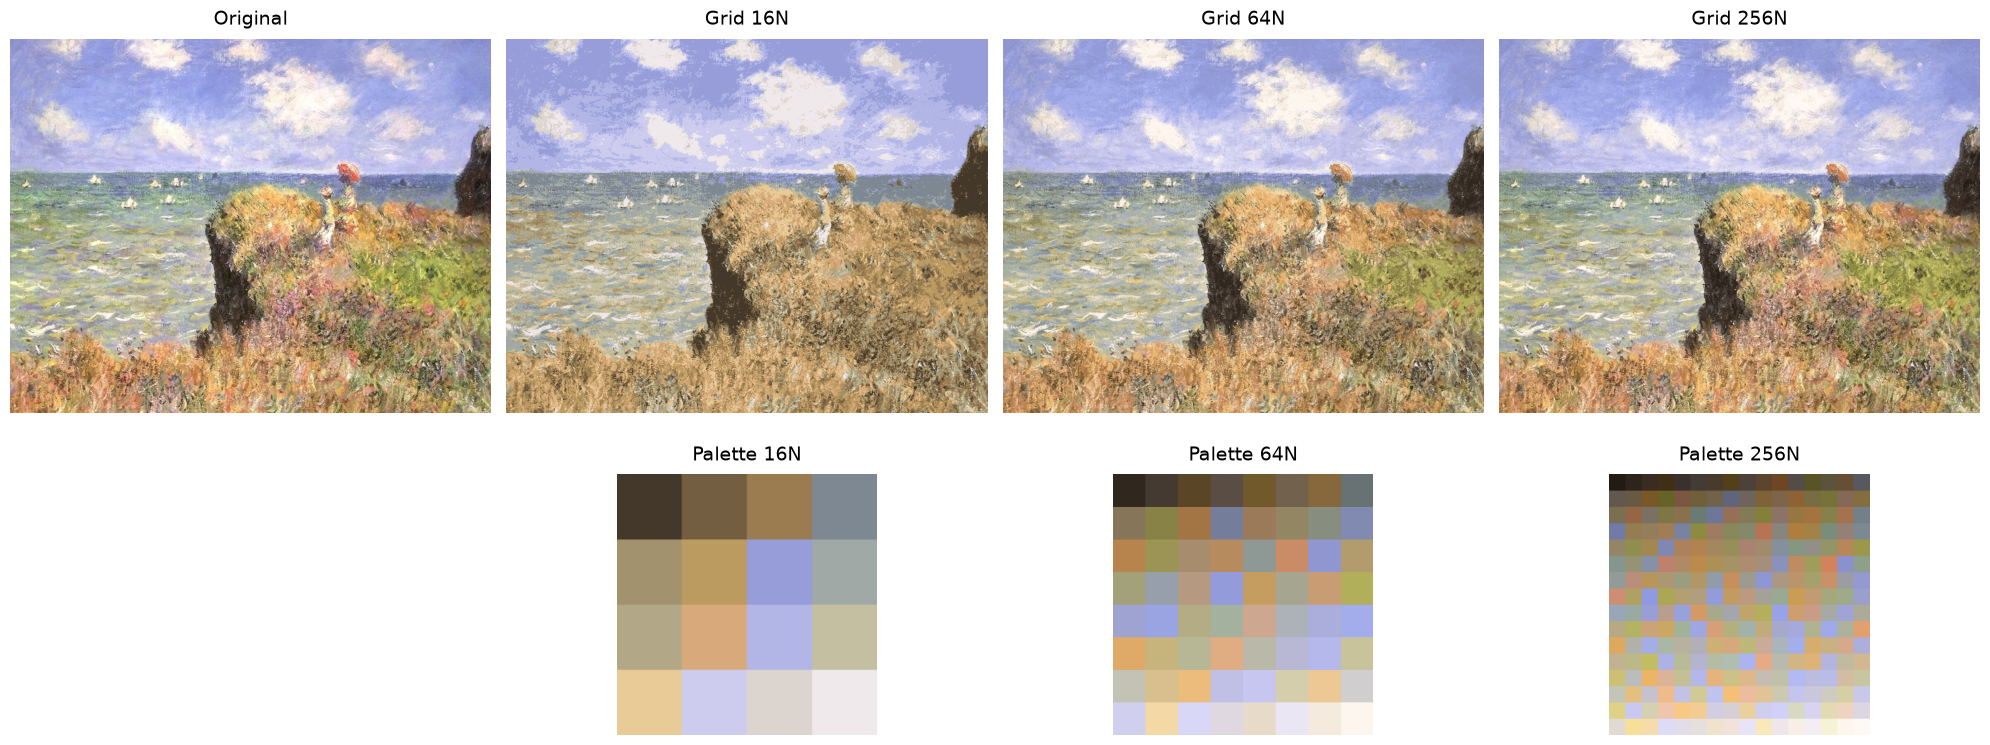
\includegraphics[width=\textwidth]{figs/gng/result-obra1.png}
    \caption{Reconstrução da Obra 1 com paleta obtida com os neurônios da rede GNG} \label{fig:gng-obra1}
\end{figure}

\begin{figure}[H]
    \centering
    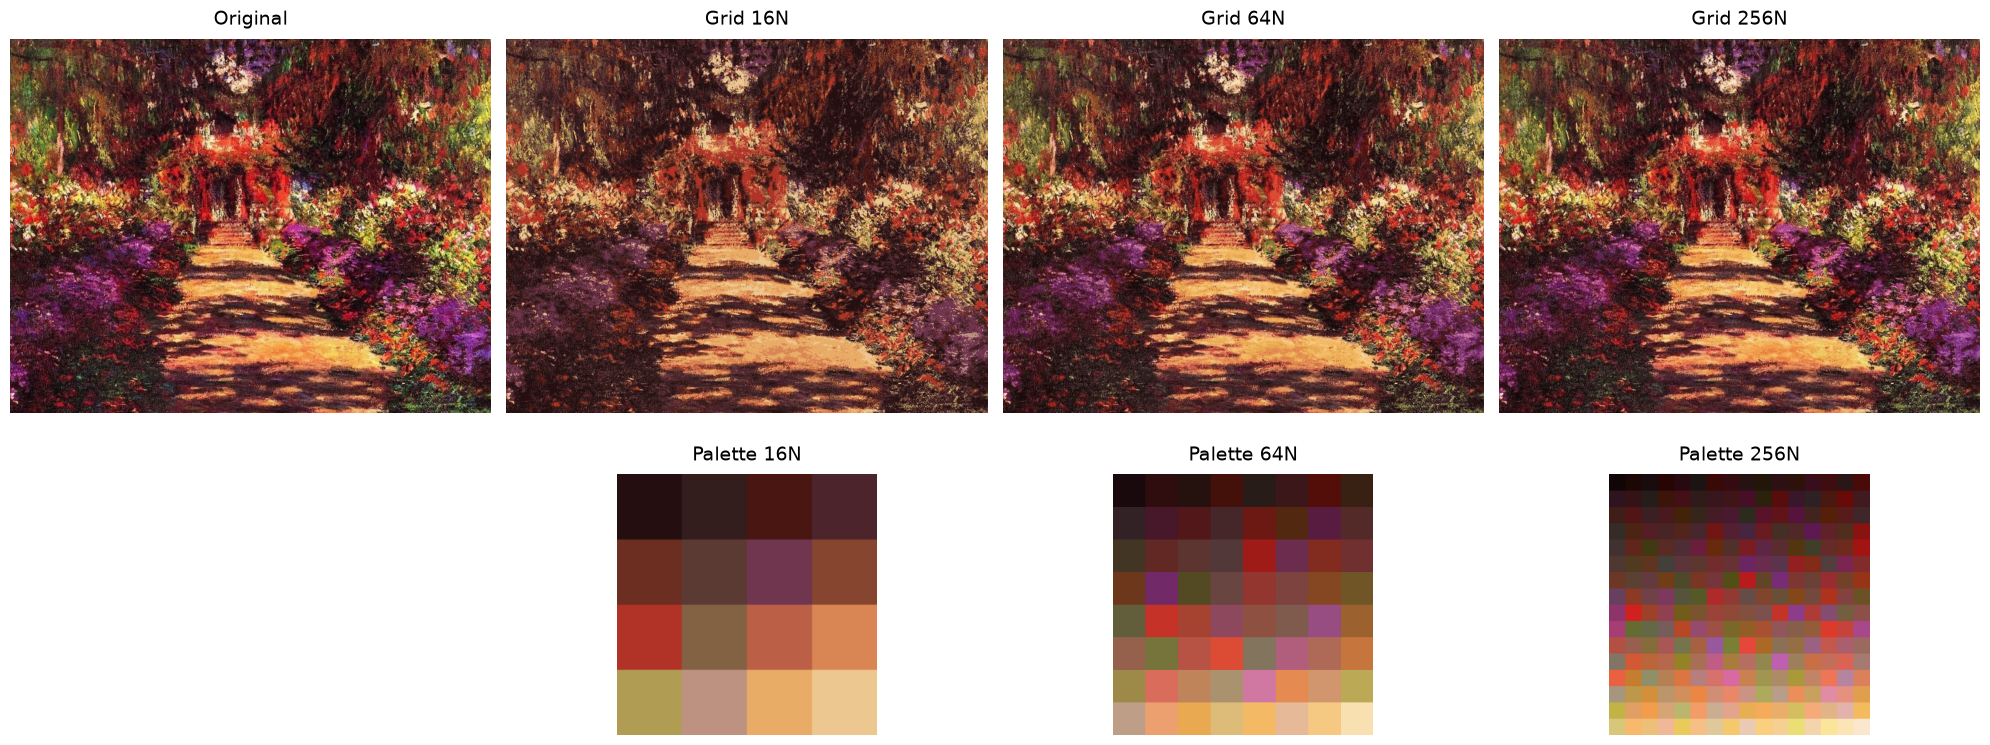
\includegraphics[width=\textwidth]{figs/gng/result-obra2.png}
    \caption{Reconstrução da Obra 2 com paleta obtida com os neurônios da rede GNG} \label{fig:gng-obra2}
\end{figure}

\begin{figure}[H]
    \centering
    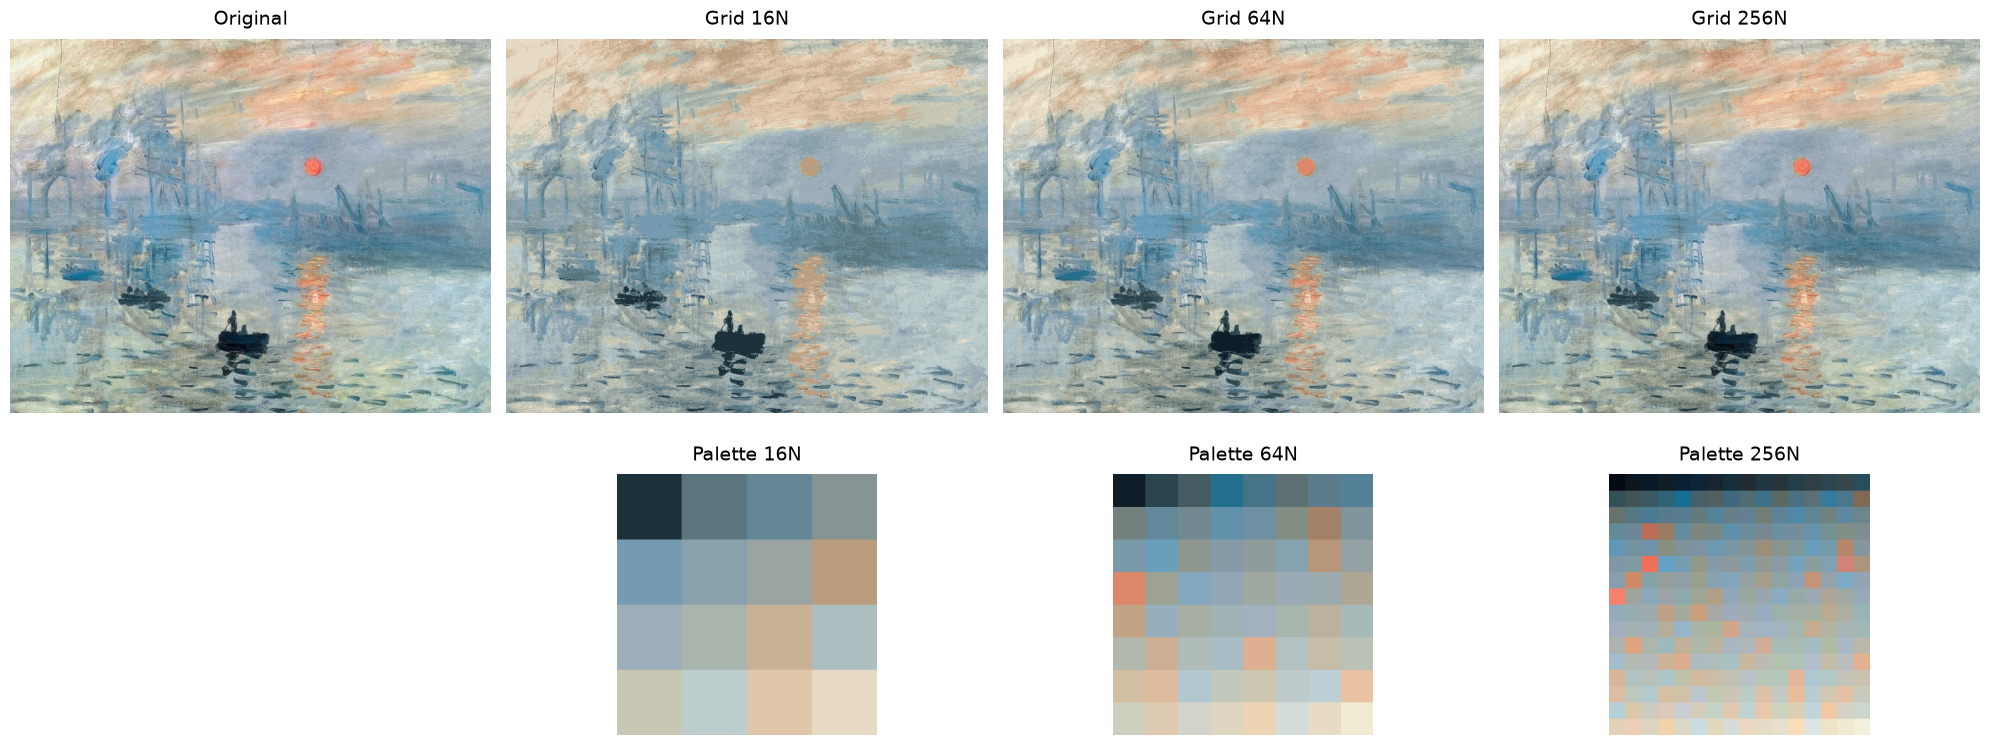
\includegraphics[width=\textwidth]{figs/gng/result-obra3.png}
    \caption{Reconstrução da Obra 3 com paleta obtida com os neurônios da rede GNG} \label{fig:gng-obra3}
\end{figure}

\begin{figure}[H]
    \centering
    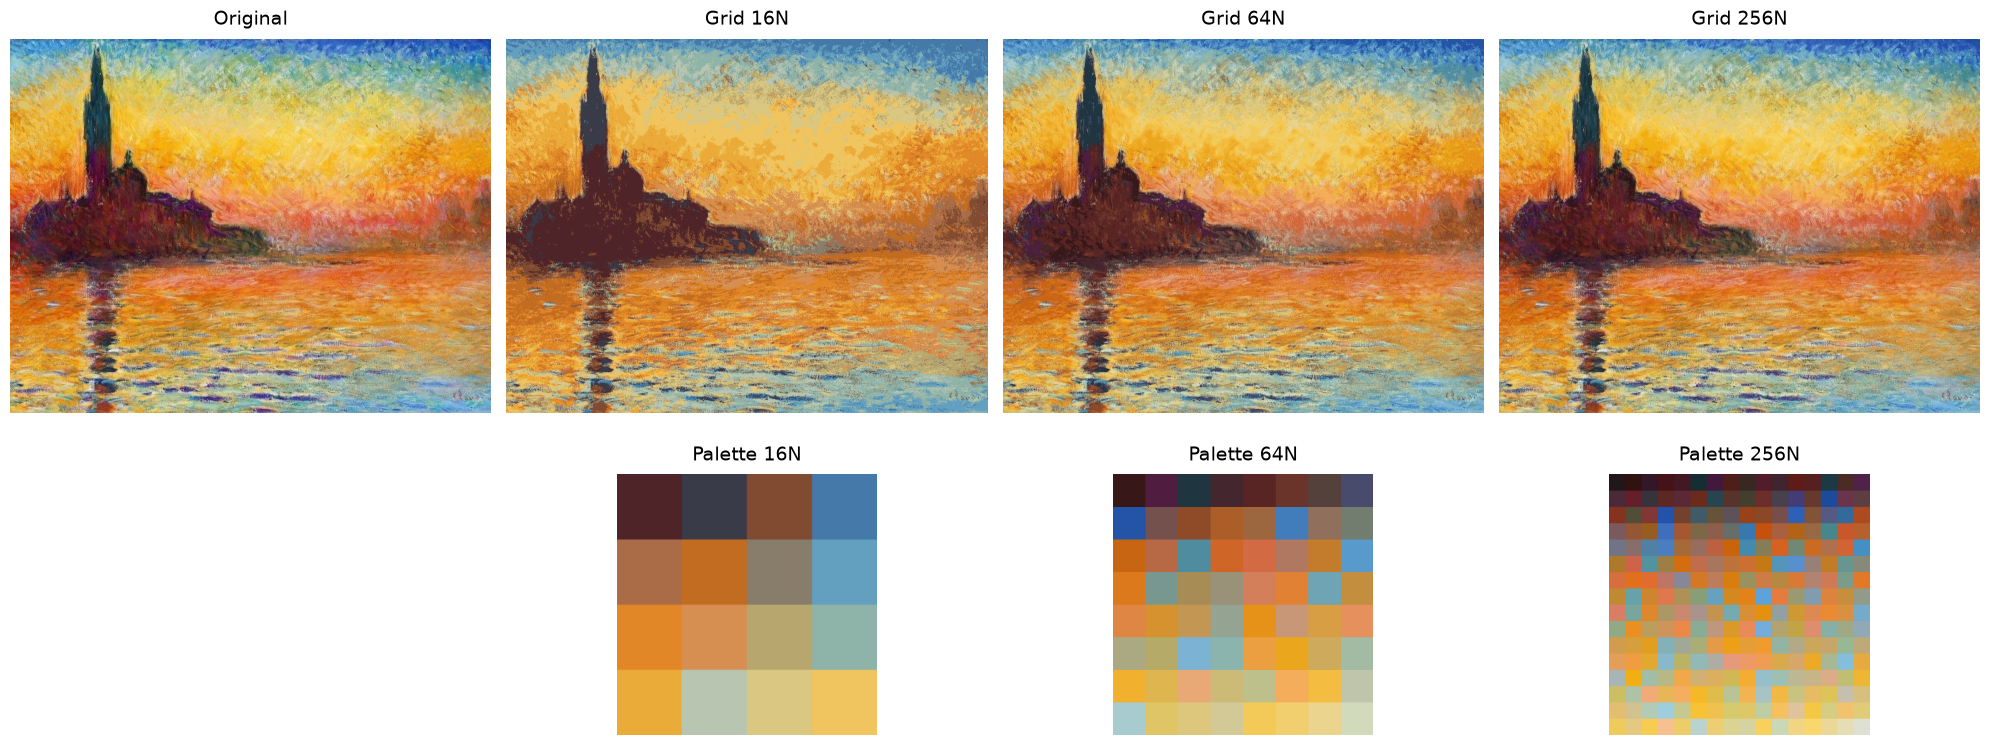
\includegraphics[width=\textwidth]{figs/gng/result-obra4.png}
    \caption{Reconstrução da Obra 4 com paleta obtida com os neurônios da rede GNG} \label{fig:gng-obra4}
\end{figure}

\begin{figure}[H]
    \centering
    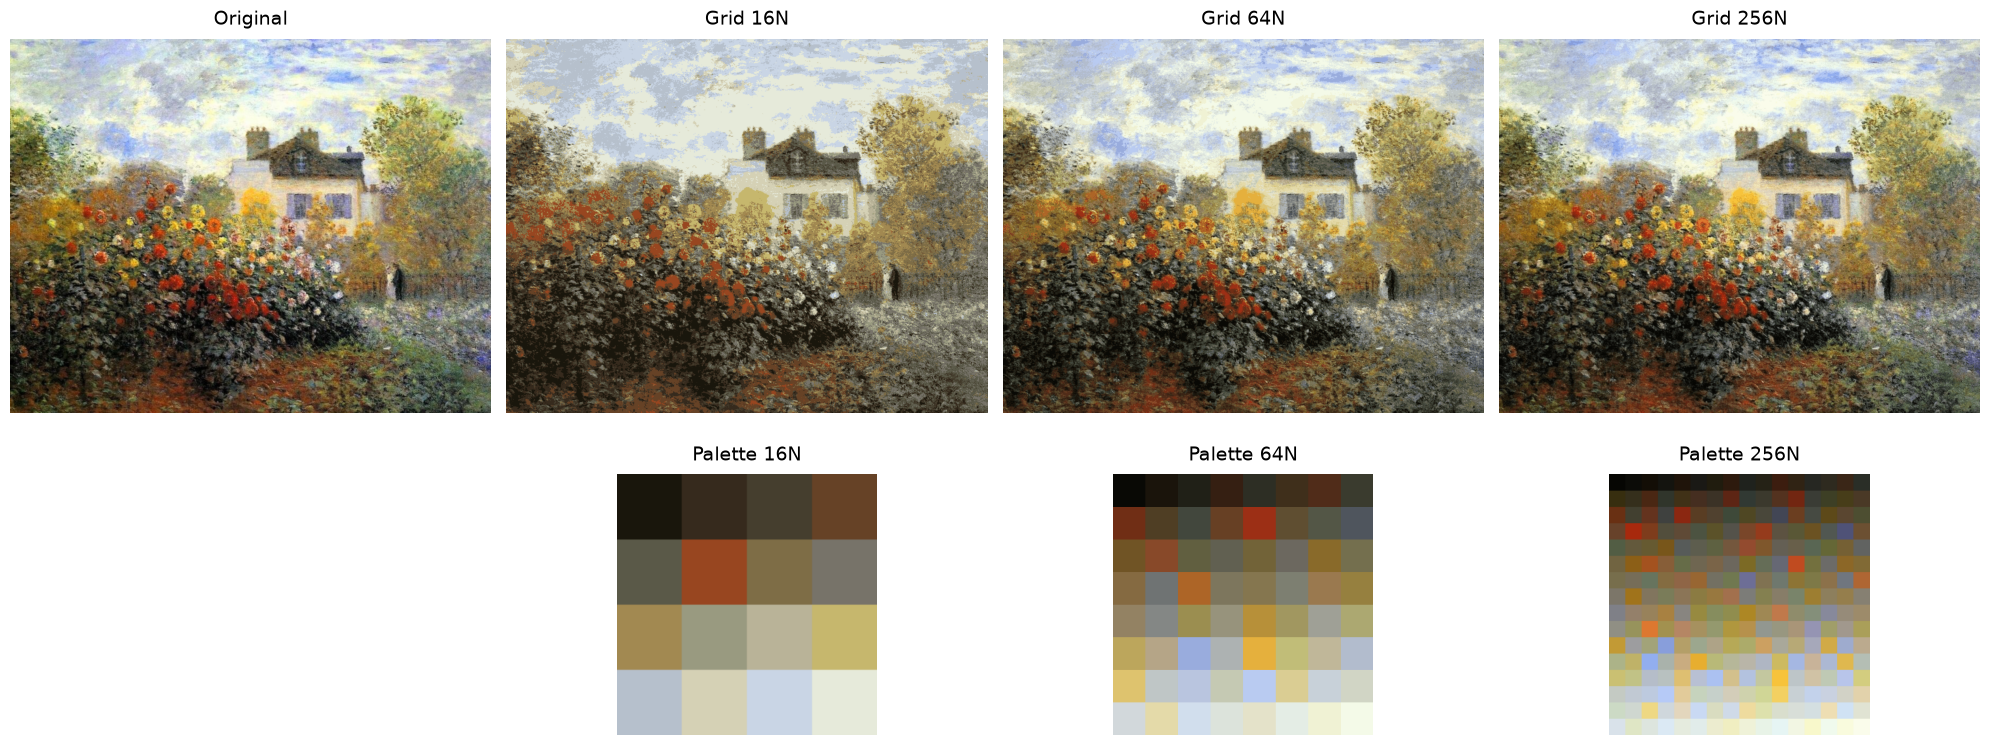
\includegraphics[width=\textwidth]{figs/gng/result-obra5.png}
    \caption{Reconstrução da Obra 5 com paleta obtida com os neurônios da rede GNG} \label{fig:gng-obra5}
\end{figure}

Assim como a rede SOM, ao aumentar a quantidade de neurônios, observou-se uma melhor representatividade de tonalidades das cores e uma correção das gradações observáveis.

\section{Resultados e Discussão}

Esta seção compara as duas redes com o mesmo número de cores na paleta e resume as conclusões do experimento. A Tabela~\ref{tab:comparacao} apresenta as médias das cinco imagens para cada tamanho de paleta, e os valores por imagem estão nas Tabelas~\ref{tab:som-resultados} e~\ref{tab:gng-resultados}.
 
\begin{table}[ht]
  \centering
  \begin{tabular}{@{}rcccccccc@{}}
    \toprule
    & \multicolumn{2}{c}{QE} & \multicolumn{2}{c}{PSNR (dB)} & \multicolumn{2}{c}{TE (\%)} & \multicolumn{2}{c}{Tempo (s)} \\
    \cmidrule(lr){2-3}\cmidrule(lr){4-5}\cmidrule(lr){6-7}\cmidrule(l){8-9}
    Cores & SOM & GNG & SOM & GNG & SOM & GNG & SOM & GNG \\
    \midrule
    $16$  & 0{,}1011 & 0{,}0746 & 22{,}74 & 26{,}51 & 0{,}904 & 0{,}096 & 61{,}4 & 35{,}0 \\
    $64$  & 0{,}0570 & 0{,}0450 & 27{,}53 & 31{,}01 & 1{,}029 & 0{,}587 & 61{,}1 & 93{,}1 \\
    $256$ & 0{,}0380 & 0{,}0283 & 31{,}05 & 35{,}06 & 1{,}185 & 1{,}016 & 61{,}5 & 324{,}5 \\
    \bottomrule
  \end{tabular}
  \caption{Médias das cinco imagens para o SOM e a GNG com o mesmo número de cores na paleta.}
  \label{tab:comparacao}
\end{table}
 
Nas duas redes, aumentar o número de neurônios reduziu o erro de quantização e elevou o PSNR em todas as imagens, com retornos decrescentes à medida que a paleta cresce. A dificuldade relativa das imagens também não dependeu da rede: as mesmas obras foram as mais fáceis e as mais difíceis de quantizar nas duas abordagens, o que indica que essa dificuldade é uma propriedade da distribuição de cores de cada pintura. Com o mesmo número de cores, a GNG obteve menor erro de quantização e maior PSNR que o SOM em todas as imagens e tamanhos de paleta, como resume a Tabela~\ref{tab:comparacao}, e isso concorda com a observação visual das reconstruções, em que a GNG conseguiu uma maior representatividade de tonalidades de cores. Uma explicação plausível, que este trabalho não testou, está na estrutura de cada rede, em que no SOM os neurônios estão presos a uma grade e são arrastados pelos vizinhos, de modo que alguns acabam em regiões pouco povoadas do espaço RGB para preservar a organização do mapa, enquanto na GNG os neurônios se movem livremente e novos neurônios são inseridos onde o erro acumulado é maior.
 
Quanto à preservação topológica, os dois erros topológicos foram baixos e o da GNG tendeu a ser menor, mas isso não indica que ela preserva melhor a topologia, pois as definições são diferentes: o SOM considera vizinhas as células adjacentes da grade, enquanto a GNG exige uma aresta direta entre os dois neurônios mais próximos, que o próprio algoritmo cria. A contribuição do SOM está na organização da paleta, que pode ser lida como um mapa de cores, o que a GNG não oferece. Em relação ao custo computacional, o tempo do SOM foi praticamente constante entre os tamanhos de grade, enquanto o da GNG cresceu de forma acentuada com o número de neurônios, sendo mais rápida com poucas cores e bem mais lenta com paletas grandes. Esses tempos, porém, não são diretamente comparáveis, pois o SOM roda em PyTorch com lotes de pixels e várias épocas, e a GNG roda em NumPy, um pixel por vez, em uma única época.
 
Os resultados devem ser lidos com algumas ressalvas. Cada combinação de imagem e tamanho foi treinada uma única vez, com semente fixa, e os hiperparâmetros de cada rede foram fixados e não variados, então não se sabe quanto cada uma melhoraria com ajuste. Além disso, QE, MSE e PSNR medem distância no espaço RGB, e não a qualidade percebida, e a avaliação visual é qualitativa. Em conclusão, as duas redes reduziram as pinturas a paletas pequenas com erro decrescente e topologia preservada. Para fidelidade de cor, a GNG foi a melhor escolha, com menor erro e maior variedade de tonalidades; o SOM é preferível quando se deseja uma paleta organizada em grade e um custo de treinamento estável mesmo para paletas grandes.
 
\end{document}